\setcounter{chapter}{1}
\chapter{Generalities on the Security Operations Center}
\label{chap:generalities}

% ========== 2.1 INTRODUCTION ==========
\section{Introduction}
\label{sec:ch2-intro}

Faced with the rise of cyber attacks, this chapter proposes a theoretical framework to understand the challenges of Security Operations Centers (SOC) and justify the SOCaaS model. We will begin by exploring key concepts related to cybersecurity. We will also clarify terminologies related To SOCs, such as logs and alerts and incidents respond , before analyzing the technologies employed in SIEM and SOAR. Finally, we will examine SOCaaS as an innovative alternative, highlighting its advantages as well as its challenges.

% ========== 2.2 GENERALITIES ON SECURITY ==========
\section{Generalities on Security}
\label{sec:security}

\subsection{Objective of Information Systems Security}
\label{subsec:cia}

Information systems security rests on three essential pillars, known as the CIA triad: Confidentiality, Integrity, and Availability. This model was designed to guide information security (infosec) policies within organizations.

Confidentiality relies on a set of rigorous rules that restrict unauthorized access to all types of data and information. Integrity, for its part, ensures the reliability and accuracy of this information. Finally, Availability constitutes a risk management approach that aims to guarantee reliable access to this data for authorized persons \cite{ref6}.

\begin{enumerate}
    \item \textbf{Confidentiality:} Confidentiality measures aim to prevent unauthorized access to sensitive information, by classifying data according to associated risks.
    \item \textbf{Integrity:} Integrity ensures that data remains consistent and reliable without unauthorized modification.
    \item \textbf{Availability:} Availability guarantees that information is accessible for authorized parties, requiring good maintenance of the systems that store and display it.
\end{enumerate}

\subsection{Vulnerability, Threat, and Risk}
\label{subsec:vulnerability}

\begin{enumerate}
    \item \textbf{Vulnerability:} A vulnerability is a weakness in an information system, system security procedures, internal controls, or implementation that could be exploited by a threat source \cite{ref7}.
    \item \textbf{Threat:} Any circumstance or event with the potential to adversely impact organizational operations, organizational assets, individuals, other organizations, or the Nation through an information system via unauthorized access, destruction, disclosure, modification of information, and/or denial of service \cite{ref7}.
    \item \textbf{Risk:} A risk represents the probability that a threat exploits a vulnerability, as well as the potential impact on the organization's assets \cite{ref7}.
\end{enumerate}

\[Risk = \frac{Threat * Vulnerability}{Countermeasures}\]

\begin{figure}[H]
\centering
\fbox{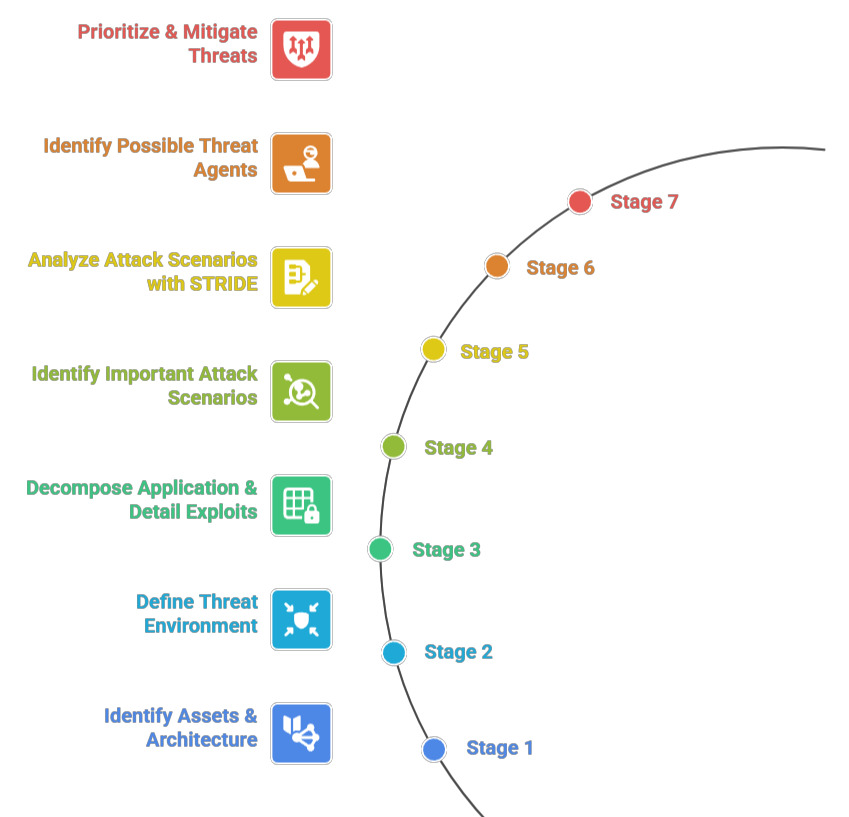
\includegraphics[width=0.75\textwidth]{figs/ThreatModeling.jpg}}
\caption{Threat Modeling}
\label{figs:threat_modeling}
\end{figure}

\subsection{Computer Threats}
\label{subsec:threats}

A cyberattack is defined as any offensive action targeting computer systems, infrastructures, or networks. It relies on various methods to steal, modify, or delete data. The term ``malware'' designates a wide range of malicious or intrusive software, such as viruses.

\begin{itemize}
    \item \textbf{Phishing:} A cyberattack that uses deceptive emails, SMS, calls, or websites to trick people into giving sensitive information or downloading malware. It exploits human weaknesses \cite{ref9}.
    \item \textbf{Ransomware:} Malicious software that holds data or a device hostage and threatens to block or destroy it if a ransom is not paid. It is widespread and can cause significant financial losses \cite{ref10}.
    \item \textbf{DoS / DDoS Attacks:} Aim to flood a server to make it inaccessible. A DoS attack comes from a single computer, while a DDoS uses multiple compromised computers to attack a target \cite{ref11}.
    \item \textbf{Trojan Horse:} A Trojan horse presents itself as a legitimate program in order to access a system \cite{ref12}.
    \item \textbf{Rootkit:} A rootkit allows cybercriminals to take control of computers while remaining hidden \cite{ref13}.
    \item \textbf{Virus:} Spreads from one computer to another, causing damage and data loss, malfunctions \cite{ref14}.
\end{itemize}

\subsection{Indicators of Compromise (IoC)}
\label{subsec:ioc}

Indicators of Compromise (IoCs) designate digital artifacts that signal an intrusion or malicious activity within a system, network, or application. They play a crucial role by enabling Security Operations (SOC) teams to detect, investigate, and respond effectively to security incidents \cite{ref15}.

\textbf{Examples of Indicators of Compromise \cite{ref16}:}

\begin{itemize}
    \item \textbf{Unusual Outbound Traffic:} Outbound traffic during off-peak hours or traffic communicating with a suspicious IP address may indicate a compromise.
    \item \textbf{High Authentication Failures:} A high rate of authentication attempts may indicate that an attacker has stolen credentials and is trying to find an account that provides network access.
    \item \textbf{Increase in Database Reads:} Whether it is an SQL injection or direct database access via an administrator account, a dump of data from database tables may indicate that an attacker has stolen data.
    \item \textbf{Suspicious Configuration Changes:} Changes could also add vulnerabilities that malware could exploit.
\end{itemize}

\subsection{Tactics, Techniques, and Procedures (TTP)}
\label{subsec:ttp}

TTPs (Tactics, Techniques, and Procedures) offer a structured framework for analyzing the methods used by cyber attackers.

\begin{itemize}
    \item \textbf{Tactic:} Tactics represent the overall objectives of an attacker.
    \item \textbf{Techniques:} Detail the specific methods used to achieve objectives.
    \item \textbf{Procedures:} Detailed descriptions of an attacker's actions, including the tools used.
\end{itemize}

\subsection{Cyber Kill Chain}
\label{subsec:killchain}

Developed by Lockheed Martin, the Cyber Kill Chain framework fits within the Intelligence Driven Defense model, designed to identify and prevent cyber intrusions. This model highlights the different stages that attackers must go through to achieve their objectives \cite{ref18}.

The seven stages of the Cyber Kill Chain enhance the visibility of an attack and deepen the understanding of an adversary's tactics, techniques, and procedures (TTPs), thus offering analysts a better perspective \cite{ref18}.

\begin{enumerate}
    \item \textbf{Reconnaissance:} During the reconnaissance phase, a malicious individual selects a target and exploits vulnerabilities and exploitable weaknesses within the network.
    \item \textbf{Weaponization:} The attacker develops an attack vector, such as malware allowing remote access, ransomware, a virus, or a worm, capable of exploiting a known vulnerability.
    \item \textbf{Delivery:} During the delivery stage, the intruder launches their attack. The specific measures adopted vary depending on the type of attack planned, such as through emails with malicious attachments or links.
    \item \textbf{Exploitation:} During the exploitation phase, the malicious code executes in the victim's system.
    \item \textbf{Installation:} After the exploitation phase, the malware installs itself, allowing the attacker to control the system.
    \item \textbf{Command and Control:} The attacker takes remote control and can navigate the network.
    \item \textbf{Actions on Objectives:} The attacker achieves their objectives, such as data theft or destruction.
\end{enumerate}

\begin{figure}[H]
\centering
\fbox{
\includegraphics[width=0.8\textwidth]{figs/CyberKillCycle.png}}
\caption{Cyber Kill Chain}
\label{fig:ch2-cyber-kill-chain}
\end{figure}

\subsection{MITRE ATT\&CK}
\label{subsec:mitre}

The MITRE ATT\&CK framework constitutes a globally accessible and continuously updated knowledge base. It is designed to model, detect, prevent, and respond to cybersecurity threats, relying on the well-documented behaviors of cybercriminals \cite{ref20}.

The MITRE ATT\&CK framework lists the tactics, techniques, and procedures (TTPs) of cybercriminals at each stage of a cyberattack lifecycle. This includes everything from the initial information gathering and attackers' planning strategies, to the final execution of the attack.

The information presented in the MITRE ATT\&CK framework enables security teams to:

\begin{itemize}
    \item Accurately simulate cyberattacks to assess the effectiveness of cyber defenses.
    \item Design more effective security policies, controls, and incident response plans.
    \item Choose and configure security technologies by optimizing the detection, prevention, and mitigation of cyber threats.
\end{itemize}

\textbf{MITRE ATT\&CK Matrices:}

\begin{enumerate}
    \item \textbf{Enterprise Matrix:} Attack techniques for enterprise infrastructures, including sub-matrices for Windows, macOS, Linux, networks, cloud, and containers \cite{ref21}.
    \item \textbf{Mobile Matrix:} Direct attack techniques on mobile devices and networks, with sub-matrices for iOS and Android \cite{ref22}.
    \item \textbf{ICS Matrix:} Techniques targeting industrial control systems, including machines, devices, sensors, and networks for various essential services \cite{ref23}.
\end{enumerate}

\subsubsection{MITRE ATT\&CK Tactics}

Each tactic in the MITRE ATT\&CK framework represents a specific objective that the attacker seeks to achieve at a given moment. These tactics are closely linked to the different stages or phases of a cyberattack. The tactics and techniques vary from one matrix to another.

\begin{figure}[H]
\centering
\fbox{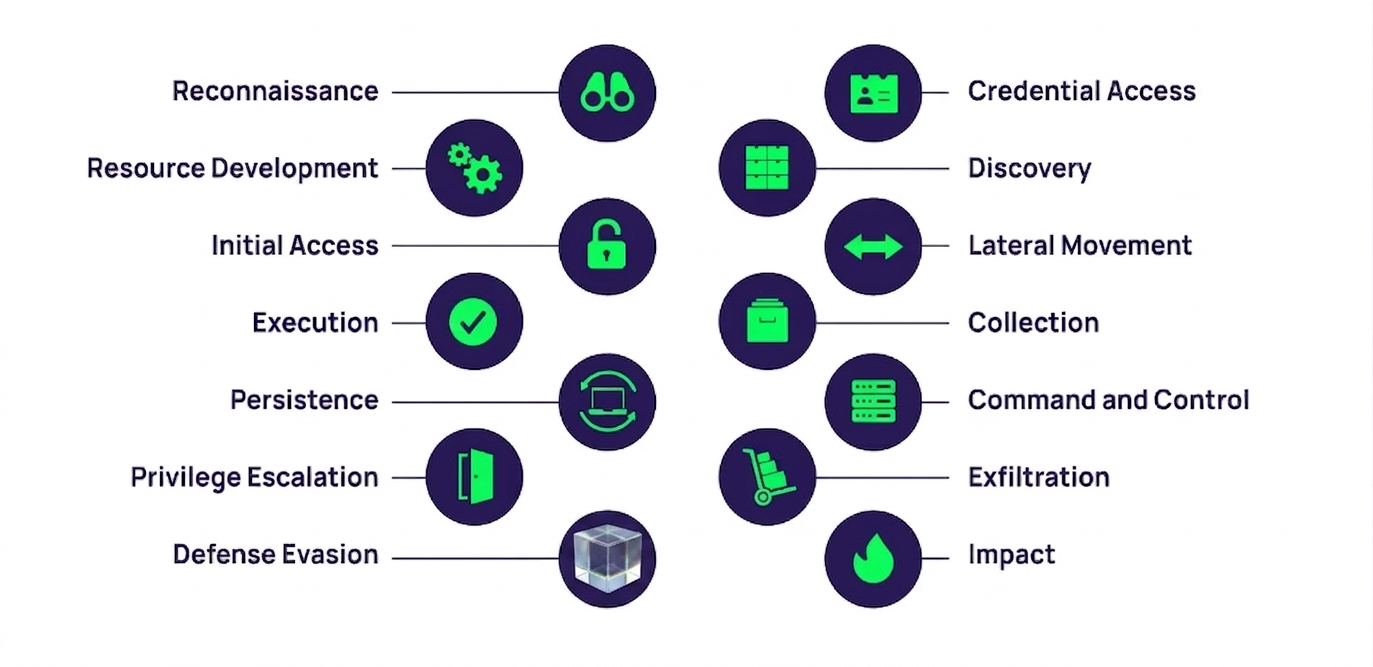
\includegraphics[width=0.9\textwidth]{figs/MITRE_ATT&CK_Enterprise_Matrix_Tactics.png}}
\caption{MITRE ATT\&CK Enterprise Matrix Tactics}
\label{fig:mitre_attack_tactics}
\end{figure}

\subsubsection{MITRE ATT\&CK Techniques}

MITRE ATT\&CK tactics illustrate the objectives that attackers seek to achieve, while MITRE ATT\&CK techniques describe the methods they employ to achieve them. For example, the techniques External Remote Services and Phishing are used within the Initial Access tactic.

This knowledge base presents the following information for each technique:

\begin{itemize}
    \item A presentation of the technique.
    \item The set of well-established sub-techniques that are linked to this technique.
    \item Examples of associated procedures, which may concern how attack groups use certain techniques, as well as the types of malware used for their implementation.
    \item Mitigations, there are security practices and software capable of blocking or managing this technique.
    \item Detection methods, generally concerning log data or other system sources that security teams or security software can monitor to identify the presence of this technique.
\end{itemize}

\subsubsection{Comparison between MITRE ATT\&CK and Cyber Kill Chain}

\begin{table}[H]
\centering
\caption{MITRE ATT\&CK VS Cyber Kill Chain}
\label{tab:mitre-vs-killchain}
\renewcommand{\arraystretch}{1.4}
\begin{tabular}{>{\raggedright\arraybackslash}p{3cm} p{5cm} p{5cm}}
\toprule
\rowcolor{tableheader}
\textbf{Criterion} & \textbf{MITRE ATT\&CK} & \textbf{Cyber Kill Chain} \\
\midrule
\textbf{Objective} & Describe attackers' TTPs. & Model the linear stages of a cyberattack. \\
\midrule
\textbf{Structure} & Dynamic matrix with 14 tactics and 200+ techniques/sub-techniques. & 7 fixed and sequential stages. \\
\midrule
\textbf{Scope} & Very detailed: Focus on concrete methods. & Macro: Describes general phases. \\
\midrule
\textbf{Flexibility} & Very flexible and capable of adapting to a variety of attack scenarios. & More linear and rigid. \\
\bottomrule
\end{tabular}
\end{table}

% ========== 2.3 TERMINOLOGIES ==========
\section{Terminologies}
\label{sec:terminologies}

\subsection{Event}
\label{subsec:event}

An event in cybersecurity is any detectable activity that occurs on a computer system, network, or application. It may be a benign, suspicious, or malicious action affecting IT resources. Events are generally recorded in logs and analyzed by monitoring tools such as a SIEM \cite{ref24}.

\textbf{Types of Events:}

\begin{itemize}
    \item \textbf{Benign Events (Normal):} Common actions that are part of normal operation (successful login, authorized file access, etc.)
    \item \textbf{Suspicious Events:} Unusual activities requiring analysis (login from an unusual location, excessive data download, etc.)
    \item \textbf{Malicious Events:} Actions signaling an attack or compromise (SQL injection, unauthorized privilege escalation, malware or ransomware detection, etc.)
\end{itemize}

\subsection{Logs}
\label{subsec:logs}

A log (or event journal) is a record file containing detailed information about the activities of a computer system, network, or application. These journals are essential for security monitoring, problem diagnosis, regulatory compliance, and incident investigation \cite{ref25} \cite{ref26}.

\textbf{Types of Logs:}

\begin{itemize}
    \item \textbf{Perimeter Device Logs:} From network security equipment such as firewalls and detection systems.
    \item \textbf{Windows Event Logs:} Windows operating system journals including user logins and security events.
    \item \textbf{Endpoint Logs:} Capture activity on computers and servers, including processes and user actions.
    \item \textbf{Application Logs:} Record events related to software, such as errors and access.
    \item \textbf{Proxy Logs:} Traces of Internet connections via a proxy server.
    \item \textbf{IoT Logs:} Journals from IoT devices to detect abnormal behaviors.
\end{itemize}

\subsection{Alert}
\label{subsec:alert}

A security alert is a notification generated automatically or manually when a suspicious event or potential threat is detected within a computer system, network, or application. It serves to warn security teams of abnormal activity that may require investigation or intervention \cite{ref27}.

Alerts are generated by cybersecurity tools such as SIEM, IDS/IPS, EDR/XDR, WAF, etc., and produced from predefined rules, artificial intelligence models, or event correlations.

\textbf{Types of Alerts:}

\begin{itemize}
    \item \textbf{True Positive:} A real threat has been detected and correctly reported. It requires intervention to mitigate the threat.
    \item \textbf{False Positive:} An alert is generated when there is no real threat. It can lead to alert overload and waste time for SOC analysts.
    \item \textbf{False Negative:} A real threat is not detected by security tools. This is the most dangerous, as an attack can go unnoticed.
    \item \textbf{True Negative:} No real threat is detected and no alert is generated. This is a normal situation, no incident to report.
\end{itemize}

\textbf{Alert Criticality Levels:}

\begin{table}[H]
\centering
\caption{Alert Criticality Levels}
\label{tab:alert-levels}
\renewcommand{\arraystretch}{1.4}
\begin{tabular}{>{\raggedright\arraybackslash}p{3cm} p{10.5cm}}
\toprule
\rowcolor{tableheader}
\textbf{Level} & \textbf{Description} \\
\midrule
\textbf{Low Alert} & Informational alerts. These events generally require no action, but it is recommended to investigate any unusual event. \\
\midrule
\textbf{Moderate Alert} & A non-standard action or unusual behavior has occurred. Investigate each case and determine the impact. \\
\midrule
\textbf{High Alert} & A potentially high-impact security event has occurred. Investigate immediately and look for secondary impacts. \\
\midrule
\textbf{Critical Alert} & Confirmed compromise requiring immediate response to avoid significant damage. \\
\bottomrule
\end{tabular}
\end{table}

\subsection{Incident}
\label{subsec:incident}

A cybersecurity incident is a proven event that compromises the confidentiality, integrity, or availability (CIA) of an organization's data, systems, or computer networks. Unlike a simple alert or a suspicious event, an incident requires immediate reaction to limit its impact and analyze its origin \cite{ref28} \cite{ref29}.

\textbf{Common Types of Incidents:}

\begin{itemize}
    \item \textbf{Unauthorized Access Attacks:} These cybersecurity incidents involve unauthorized attempts by cybercriminals to access systems or data using authorized user accounts.
    \item \textbf{Malware-Related Incidents:} These incidents involve malicious software that compromises computer systems (Ransomware, Trojan, Worms, Spyware, etc.)
    \item \textbf{Denial of Service Attacks:} Attempts to overload systems to make them unavailable.
    \item \textbf{Phishing Incidents:} Attacks that aim to deceive users to steal sensitive information.
    \item \textbf{Web Application Incidents:} This event occurs when a web application is used in an attack.
\end{itemize}

\subsection{Comparison between Event, Alert, and Incident}

\begin{table}[H]
\centering
\caption{Comparison between Event, Alert, and Incident}
\label{tab:event-alert-incident}
\renewcommand{\arraystretch}{1.4}
\begin{tabular}{>{\raggedright\arraybackslash}p{2.5cm} p{3.5cm} p{3.5cm} p{3.5cm}}
\toprule
\rowcolor{tableheader}
\textbf{Criterion} & \textbf{Event} & \textbf{Alert} & \textbf{Incident} \\
\midrule
\textbf{Nature} & Informational, may be benign or suspicious. & Indicator of a potential security problem. & Proven problem requiring immediate response. \\
\midrule
\textbf{Detection} & Recorded in system logs. & Generated automatically by cybersecurity tools. & Confirmed by SOC analysts after alert investigation. \\
\midrule
\textbf{Response} & No action required in general. & Requires analysis to determine if it is a false positive or a real problem. & Immediate action required to contain and remediate the threat. \\
\bottomrule
\end{tabular}
\end{table}

\subsection{Container}
\label{subsec:container}

Containers are technologies that allow packaging and isolating applications, integrating their entire execution environment. This approach simplifies the transfer of applications between different environments while preserving all their functionalities.

Containers offer numerous advantages for both developers and system administrators:

\begin{itemize}
    \item \textbf{Scalability:} Developers can easily adapt the infrastructure size according to application needs.
    \item \textbf{Portability:} Facilitate migration from one infrastructure to another without requiring substantial application modifications.
    \item \textbf{Resilience:} A failure in one container will not affect other running containers. It is possible to configure containers to restart automatically in case of failure, thus ensuring continuous availability.
\end{itemize}

% ========== 2.4 SECURITY OPERATIONS CENTER (SOC) ==========
\section{Security Operations Center (SOC)}
\label{sec:soc}

A Security Operations Center (SOC) is a team of experts dedicated to the proactive monitoring of an organization's security. It is also a command center responsible for supervising all information systems, including servers, applications, networks, workstations, data centers, and other endpoints \cite{ref30} \cite{ref31}.

The SOC ensures continuous monitoring, assesses the security posture of the infrastructure, detects potential and existing threats, and orchestrates incident response. In addition to threat monitoring and response, it implements security protocols and measures aimed at strengthening the cybersecurity posture and preventing future attacks \cite{ref30} \cite{ref31}.

\subsection{SOC Activities}
\label{subsec:soc-activities}

SOC activities are divided into three main categories \cite{ref32}:

\subsubsection{Preparation, Planning, and Prevention}

\begin{itemize}
    \item \textbf{Asset Inventory:} List the elements to protect, such as applications and servers.
    \item \textbf{Preventive Maintenance:} Apply patches and update firewalls.
    \item \textbf{Incident Response Planning:} Develop a plan defining activities, roles, and responsibilities in case of threat or incident.
    \item \textbf{Regular Testing:} Assess vulnerabilities and adjust security policies.
\end{itemize}

\subsubsection{Monitoring, Detection, and Response}

\begin{itemize}
    \item \textbf{Continuous Monitoring:} Monitor IT infrastructure to detect suspicious activities.
    \item \textbf{Log Management:} Analyze logs to identify anomalies.
    \item \textbf{Threat Detection:} Use SIEM to monitor alerts and identify threats.
\end{itemize}

\subsubsection{Recovery, Improvement, and Compliance}

\begin{itemize}
    \item \textbf{Recovery and Remediation:} After an incident, the SOC eliminates the threat and restores affected assets.
    \item \textbf{Post-Incident Analysis and Improvement:} Analyze the incident to improve processes, policies, and security tools.
    \item \textbf{Compliance Management:} Ensure everything is compliant with data privacy regulations such as GDPR, CCPA, PCI DSS, ISO 27001, and HIPAA.
\end{itemize}

\subsection{SOC Components}
\label{subsec:soc-components}

A SOC consists of several essential components enabling the monitoring, detection, and response to cybersecurity incidents. These components can be classified into three categories: People, Processes, and Technologies \cite{ref34}.

\subsubsection{People}

The first and most important aspect of a security operations team is the people. The human element is at the heart of a SOC's success. A security operations center is only as effective as the people who run it. A SOC team is a diverse group of professionals, each having a specific role to play.

\begin{table}[H]
\centering
\caption{Roles and Responsibilities of the SOC Human Component}
\label{tab:soc-roles}
\renewcommand{\arraystretch}{1.4}
\begin{tabular}{>{\raggedright\arraybackslash}p{3cm} p{10.5cm}}
\toprule
\rowcolor{tableheader}
\textbf{Role} & \textbf{Responsibility} \\
\midrule
\textbf{SOC Analyst} & Continuously monitor security alerts; Triage and classify incidents; Perform initial threat analysis; Escalate critical incidents. \\
\midrule
\textbf{Incident Responder} & Investigate confirmed incidents; Contain and eradicate threats; Coordinate system restoration. \\
\midrule
\textbf{Threat Hunter} & Actively search for undetected threats; Analyze attacker TTPs; Improve detection rules. \\
\midrule
\textbf{SOC Manager} & Supervise daily operations; Manage communication with stakeholders; Coordinate security audits. \\
\bottomrule
\end{tabular}
\end{table}

\subsubsection{Processes}

The second most important aspect of a security operations center concerns the processes involved. These processes include effective workflows and procedures. When an alert is triggered, workflows follow a process that includes:

\begin{itemize}
    \item \textbf{Alert Triage:} Classification of alerts by priority (low, medium, critical).
    \item \textbf{Investigation:} Analysts examine suspicious activities more deeply to determine if they are security incidents.
    \item \textbf{Containment:} If a security incident is confirmed, the SOC team takes measures to isolate it and minimize damage.
    \item \textbf{Remediation:} Measures are taken to correct vulnerabilities and prevent future incidents.
\end{itemize}

\subsubsection{Technologies}

Tools and technology constitute the foundation on which a security operations center builds its defenses. Tools collect, correlate, and analyze data, equipping the SOC team with real-time threat monitoring and detection capabilities. In the following section, we will see how these technologies strengthen a security operations center.

% ========== 2.5 SOC TECHNOLOGIES AND TOOLS ==========
\section{SOC Technologies and Tools}
\label{sec:technologies}

The SOC relies on an advanced technological infrastructure to monitor, detect, analyze, and respond to threats. These technologies are essential to ensure effective and proactive cybersecurity.

\subsection{Security Information and Event Management (SIEM)}
\label{subsec:siem}

A SIEM is a key technological solution in a SOC. It enables the collection, analysis, correlation, and archiving of logs from various information systems such as servers, network equipment, and security systems. Thanks to its central role, it helps detect, investigate, and respond to security threats in real time \cite{ref35} \cite{ref36}.

The SIEM itself relies on 2 components:

\begin{itemize}
    \item \textbf{SIM (Security Information Management):} Stores and analyzes logs over the long term for compliance and forensic analysis.
    \item \textbf{SEM (Security Event Management):} Analyzes events in real time and triggers alerts in case of threat.
\end{itemize}

\subsubsection{SIEM Functionalities}

\begin{itemize}
    \item \textbf{Log Management:} Collects real-time log data from various devices (endpoints, firewalls, antivirus, etc.) and cloud environments.
    \item \textbf{Event Correlation and Analysis:} Uses advanced analytics to identify data patterns and identify threats.
    \item \textbf{Incident Monitoring and Security Alerts:} A centralized dashboard allows monitoring activity and managing alerts.
    \item \textbf{Compliance Management:} Helps collect and verify compliance data within the company.
\end{itemize}

\subsubsection{SIEM Advantages}

\begin{itemize}
    \item \textbf{Efficiency:} Provides a comprehensive view of data and facilitates collaboration to counter threats.
    \item \textbf{User and Application Monitoring:} Tracks all network activities, ensuring transparency and threat detection.
    \item \textbf{Real-time Identification:} Analyzes data to identify anomalies indicating security problems.
    \item \textbf{Compliance:} Ensures compliance with regulations according to sectors and regions (HIPAA, GDPR, PCI-DSS, etc.).
\end{itemize}

\subsection{Security Orchestration, Automation and Response (SOAR)}
\label{subsec:soar}

SOAR is a set of compatible software that offers an organization the ability to gather data on cybersecurity threats and respond to security incidents to optimize the efficiency of security operations. A SOAR platform consists of three essential elements: orchestration, automation, and response \cite{ref35} \cite{ref36}.

\begin{itemize}
    \item \textbf{Orchestration:} Connects various internal and external tools via integrations such as vulnerability scanners.
    \item \textbf{Automation:} Allows executing previously manual tasks, such as vulnerability analysis by following Playbooks.
    \item \textbf{Response:} Together, orchestration and automation strengthen an organization's response to security threats.
\end{itemize}

\subsubsection{SOAR Elements}

\begin{itemize}
    \item \textbf{Security Orchestration and Automation (SOA):} This element ensures the management of orchestration and automation of workflows using playbooks and processes.
    \item \textbf{Security Incident Response Platform (SIRP):} This platform enables centralized management of security incidents, offering complete visibility on threats.
    \item \textbf{Threat Intelligence Platform (TIP):} Provides information on attackers' tactics, techniques, and procedures (TTPs), thus helping SOC teams develop appropriate response strategies.
\end{itemize}

\subsubsection{SOAR Advantages}

\begin{itemize}
    \item \textbf{Optimize Time Management and Efficiency:} SOAR adoption increases productivity by freeing up team members' time for other objectives.
    \item \textbf{Flexibility:} SOAR adapts to the specific needs of each organization and evolves with the existing security system.
    \item \textbf{Manage Incidents More Effectively:} SOAR infrastructure enables rapid response to threats, reducing errors and resolution time.
    \item \textbf{Streamlined Operations:} Standardized procedures and playbooks help SecOps teams manage more threats quickly.
\end{itemize}

\subsubsection{Relationship between SIEM and SOAR}

Both platforms are complementary and can collaborate effectively to optimize security operations within a company. SIEM collects data and generates alerts for security personnel. SOAR uses this information to automate responses and integrates AI to predict similar threats. Together, they optimize security operations \cite{ref36}.

\subsection{Extended Detection and Response (XDR)}
\label{subsec:xdr}

A unified security incident detection and response platform that automatically collects and correlates data from various security components (endpoints, network, cloud, email, etc.) \cite{ref37}.

XDR enables security teams to quickly and effectively identify and eliminate threats across various domains, all from a unified solution.

\subsubsection{XDR Operation}

\begin{itemize}
    \item \textbf{Ingestion:} Gathers and normalizes data from different sources.
    \item \textbf{Detection:} Analyzes and correlates data to detect threats with AI and ML.
    \item \textbf{Response:} Classifies threats by severity to facilitate their analysis and automates responses.
\end{itemize}

\subsubsection{XDR Advantages}

\begin{itemize}
    \item \textbf{Improved Visibility:} Provides in-depth understanding of the security environment by integrating data from various sources, enabling the description of invisible threats.
    \item \textbf{Improved Productivity and Efficiency:} Automates repetitive tasks and facilitates self-healing, reducing analyst workload.
    \item \textbf{Improved Incident Prioritization:} Identifies critical incidents requiring rapid intervention.
\end{itemize}

\subsubsection{Comparison between SIEM, SOAR, and XDR}

\begin{table}[H]
\centering
\caption{Comparison between SIEM, SOAR, and XDR}
\label{tab:siem-soar-xdr}
\footnotesize
\setlength{\tabcolsep}{3pt}
\renewcommand{\arraystretch}{1.3}
\begin{tabular}{>{\RaggedRight\arraybackslash}p{2.5cm} p{3.5cm} p{3.5cm} p{3.5cm}}
\toprule
\rowcolor{tableheader}
\textbf{Criterion} & \textbf{SIEM} & \textbf{SOAR} & \textbf{XDR} \\
\midrule
\textbf{Main Role} & Log collection and correlation & Orchestration and automation & Extended detection and response \\
\midrule
\textbf{Data Source} & IT logs (firewalls, servers, network) & Data from existing tools & Endpoints, network, cloud, identities, emails \\
\midrule
\textbf{Automation} & Low & High & High \\
\midrule
\textbf{Advanced Correlation} & Limited & Based on playbooks & Multi-layered (endpoint, network, cloud, etc.) \\
\midrule
\textbf{Threat Management} & Reactive & Reactive and automated & Proactive across the entire IT environment \\
\midrule
\textbf{Complexity} & High & High & Medium \\
\bottomrule
\end{tabular}
\end{table}

\subsection{Intrusion Detection System \& Intrusion Prevention System (IDS / IPS)}
\label{subsec:ids-ips}

\subsubsection{Intrusion Detection System (IDS)}

An IDS is a monitoring system that analyzes network traffic to detect possible attacks or suspicious behaviors. It functions as an alarm system that warns the administrator without directly intervening. It enables capturing network traffic, analyzing packets via rules and signatures, and generating an alert in case of suspicious activity \cite{ref35}.

\textbf{Types of IDS:}

\begin{itemize}
    \item \textbf{Network Intrusion Detection System (NIDS):} Monitors overall network traffic and alerts in case of abnormal behaviors.
    \item \textbf{Host Intrusion Detection System (HIDS):} Examines network packets on a specific host to detect malicious activities.
    \item \textbf{Protocol-Based Intrusion Detection System (PIDS):} Analyzes traffic between a server and a client according to specific protocols.
    \item \textbf{Application Protocol-based Intrusion Detection System (APIDS):} Monitors communication to identify security flaws in application protocols.
\end{itemize}

\begin{figure}[H]
\centering
\fbox{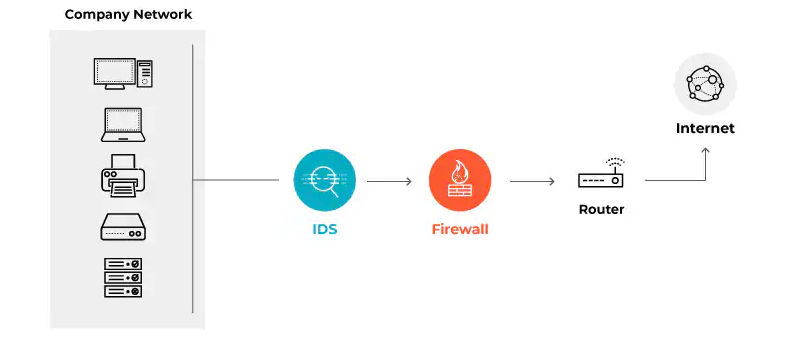
\includegraphics[width=0.8\textwidth]{figs/IDS_Location.png}}
\caption{IDS Location}
\label{fig:ids_location}
\end{figure}

\subsubsection{Intrusion Prevention System (IPS)}

In contrast, an IPS, often integrated with IDS, goes further by taking active measures to block or mitigate these threats in real time. It can automatically reject malicious data packets, block suspicious traffic sources. It enables capturing network traffic, identifying threats through signatures, and taking immediate measures (block IP, cut connection, etc.) \cite{ref35}.

\textbf{Types of IPS:}

\begin{itemize}
    \item \textbf{Network-Based Intrusion Prevention System (NIPS):} Monitors all network traffic to detect and eliminate security violations.
    \item \textbf{Host-Based Intrusion Prevention System (HIPS):} Installed on endpoints to monitor incoming and outgoing traffic of that device only.
    \item \textbf{Network Behavior Analysis (NBA):} Detects unusual traffic flows and blocks denial of service attacks.
    \item \textbf{Wireless Intrusion Prevention System (WIPS):} Monitors wireless network traffic.
\end{itemize}

\begin{figure}[H]
\centering
\fbox{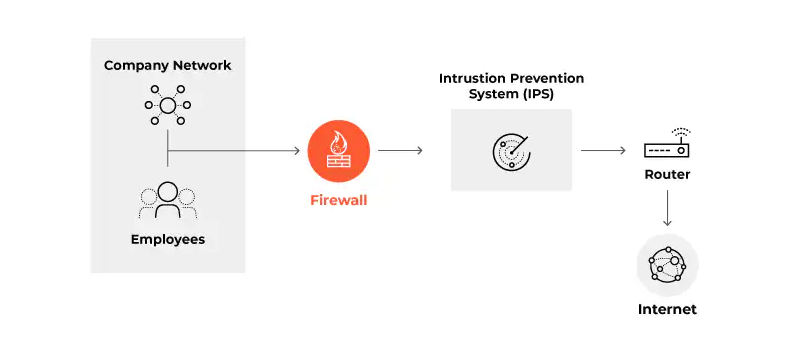
\includegraphics[width=0.8\textwidth]{figs/IPS_Location.png}}
\caption{IPS Location}
\label{fig:ips_location}
\end{figure}

\subsubsection{Comparison between IDS and IPS}

\begin{table}[H]
\centering
\caption{Comparison between IDS and IPS}
\label{tab:ids-ips}
\footnotesize
\setlength{\tabcolsep}{3pt}
\renewcommand{\arraystretch}{1.3}
\begin{tabular}{>{\RaggedRight\arraybackslash}p{3cm} p{5cm} p{5cm}}
\toprule
\rowcolor{tableheader}
\textbf{Criterion} & \textbf{IDS} & \textbf{IPS} \\
\midrule
\textbf{Main Role} & Detect and signal intrusions & Detect and block intrusions \\
\midrule
\textbf{Action} & Generates an alert in case of anomaly & Actively blocks detected threats \\
\midrule
\textbf{Human Intervention} & Requires human analysis for decision-making & Automated, makes real-time decisions \\
\midrule
\textbf{Position in Network} & In listening mode, often connected in parallel & In active mode, often inline in traffic \\
\midrule
\textbf{Impact on Traffic} & No impact on network traffic & May slightly slow traffic due to filtering \\
\midrule
\textbf{False Positive Management} & Generates alerts, risk of high number of false positives & May wrongly block legitimate traffic if poorly configured \\
\bottomrule
\end{tabular}
\end{table}

% ========== 2.6 SOC CHALLENGES ==========
\section{SOC Challenges}
\label{sec:challenges}

SOCs face several major challenges that can compromise their effectiveness. These challenges are related to the increasing complexity of IT environments, the evolution of threats, and operational constraints. Here is an analysis of the main challenges facing SOCs \cite{ref38} \cite{ref39}:

\subsection{Alert Fatigue}
\label{subsec:alert-fatigue}

Alert fatigue is a common phenomenon in SOCs, where analysts are overwhelmed by an excessive volume of alerts, many of which are false positives. This alert overload can lead to:

\begin{itemize}
    \item \textbf{Decreased vigilance:} Analysts may become less attentive to alerts, increasing the risk of missing real threats.
    \item \textbf{Decreased efficiency:} Time spent processing irrelevant alerts reduces analysts' ability to focus on critical threats.
    \item \textbf{Impact on morale:} Alert fatigue can lead to stress and frustration among analysts, which can affect their performance and engagement.
\end{itemize}

\subsection{Complexity of Environments}
\label{subsec:complexity}

With the increasing adoption of environments, especially hybrid environments, SOCs must monitor geographically and technologically dispersed systems. This complexity poses several challenges:

\begin{itemize}
    \item \textbf{Log Collection and Correlation:} Tools are needed to manage large amounts of data in real time.
    \item \textbf{Limited Visibility:} SOCs may have limited visibility over certain activities in cloud environments.
\end{itemize}

\subsection{Cybersecurity Skills Shortage}
\label{subsec:skills-shortage}

The shortage of qualified cybersecurity professionals is a major challenge for SOCs. SOC analysts must possess in-depth technical skills to analyze alerts, investigate incidents, and configure security tools. However, the lack of qualified personnel can lead to:

\begin{itemize}
    \item \textbf{Work Overload:} Existing analysts may be overwhelmed by the volume of alerts to process, increasing the risk of errors or delays in incident response.
    \item \textbf{Difficulty in Keeping Skills Up-to-Date:} Threats evolve rapidly, and analysts must constantly train to stay current on new attack techniques and security tools.
\end{itemize}

\subsection{Evolution of Threats and Sophisticated Attacks}
\label{subsec:evolved-threats}

Cyber threats are constantly evolving, with increasingly sophisticated and targeted attacks. SOCs must face challenges such as:

\begin{itemize}
    \item \textbf{Zero-Day Attacks:} These attacks exploit unknown flaws without a patch.
    \item \textbf{Advanced Persistent Threats (APT):} These attacks, orchestrated by state entities or organized groups, can hide for months or even years.
\end{itemize}

\subsection{Compliance and Regulation}
\label{subsec:compliance}

Organizations are subject to strict data protection regulations (such as GDPR in Europe or CCPA in California). SOCs must ensure that their monitoring and incident response activities comply with these regulations. This involves:

\begin{itemize}
    \item \textbf{Log Management:} Logs must be retained for a defined period and be accessible for compliance audits.
    \item \textbf{Sensitive Data Protection:} SOCs must guarantee that collected and analyzed data is protected against unauthorized access.
\end{itemize}

\subsection{Costs and Return on Investment (ROI)}
\label{subsec:costs}

Establishing and operating a SOC represents a significant investment in terms of costs (infrastructure, tools, personnel). Organizations must justify this investment by demonstrating tangible return on investment (ROI). However, measuring a SOC's effectiveness can be difficult, as it is often challenging to quantify avoided incidents or potential damages.

% ========== 2.7 SOCaaS ==========
\section{Security Operations Center as a Service (SOCaaS)}
\label{sec:socaas}

A Security Operations Center as a Service (SOCaaS) is a security model in which a third-party provider manages and maintains a complete SOC, accessible via a cloud subscription \cite{ref40} \cite{ref41}.

SOCaaS offers all the security functions of a traditional internal SOC, including continuous monitoring, log management, threat detection, incident response, remediation, compliance, etc. \cite{ref40} \cite{ref41}.

The provider also assumes responsibility for all the people, processes, and technologies necessary to enable these services and guarantee 24/7 support \cite{ref40} \cite{ref41}.

\subsection{SOCaaS Advantages}
\label{subsec:socaas-advantages}

Compared to a traditional on-premises SOC, SOCaaS offers companies several notable advantages. Here are some of them \cite{ref41}:

\begin{itemize}
    \item \textbf{Reduce Costs:} Subscribing to a SOCaaS subscription is cheaper than purchasing all the tools necessary for an effective SOC team.
    \item \textbf{Faster Identification and Remediation:} Thanks to recent tools and qualified personnel, security incidents are processed more quickly.
    \item \textbf{Reduces Security Risks:} 24/7 monitoring allows rapid identification of intrusions before they spread.
    \item \textbf{Scalability and Flexibility:} Services can adapt to the company's needs.
    \item \textbf{Improved Maturity:} External experts strengthen security without weighing down the budget.
    \item \textbf{Keep Your Security Up-to-Date:} Access to the latest technologies and security practices.
\end{itemize}

\subsection{SOCaaS Challenges}
\label{subsec:socaas-challenges}

Although outsourcing security operations offers many strengths, it can also generate challenges and limitations.

\begin{itemize}
    \item \textbf{Onboarding Process:} The provider must configure security solutions in the client's environment before starting to offer its services. This can be long and complex, exposing the company to risks.
    \item \textbf{Data Sharing and Storage:} The SOCaaS provider needs access to sensitive data to combat threats, which can increase the risk of data leaks.
    \item \textbf{Compliance:} Compliance must remain the organization's responsibility, as certain tasks are not compatible with a third-party provider.
\end{itemize}
$a revoir$
\subsection{Comparison between SOCaaS and Internal SOC}

\begin{table}[H]
\centering
\caption{Comparison between SOCaaS and Internal SOC}
\label{tab:socaas-vs-internal}
\renewcommand{\arraystretch}{1.4}
\begin{tabular}{>{\raggedright\arraybackslash}p{3cm} p{5cm} p{5cm}}
\toprule
\rowcolor{tableheader}
\textbf{Criterion} & \textbf{Internal SOC} & \textbf{SOCaaS} \\
\midrule
\textbf{Cost} & High investment (tools, technologies, salaries). & Monthly subscription / pay-per-use. \\
\midrule
\textbf{Expertise} & Internal recruitment and training. & Expertise provided by the provider. \\
\midrule
\textbf{Infrastructure} & On-premises servers and tools. & Cloud platform managed by the provider. \\
\midrule
\textbf{Response Time} & Depends on internal team availability. & Guaranteed response time (SLA). \\
\bottomrule
\end{tabular}
\end{table}

% ========== 2.8 SOCaaS SOLUTION ==========
\section{SOCaaS Solution}
\label{sec:socaas-solution}

Building on the theoretical foundations established in this chapter, we now address the central operational objective of this thesis: to design and deploy an open-source SOCaaS that is efficient, accessible, and specially adapted to the needs of businesses. Driven by an ambition for technological sovereignty and cyber inclusion, this project will transform concepts into tangible reality. A credible alternative to proprietary solutions, where security effectiveness rhymes with ease of use and cost control. The following pages will unveil our concrete architecture, the result of a rigorous selection of tools and modeling centered on real field challenges.

% ========== 2.9 CONCLUSION ==========
\section{Conclusion}
\label{sec:ch2-conclusion}

This chapter covered the theoretical and practical foundations of SOCs. We explored the key concepts of cybersecurity, clarified SOC terminologies, and detailed its technologies. The structural challenges of traditional SOCs highlighted the need for an innovative model. SOCaaS emerges as a promising alternative, offering flexibility and scalability, despite persistent challenges such as trust in the cloud. These elements constitute the basis for designing a SOCaaS solution adapted to current needs, as proposed by this project.
\begin{comment}
% ========== BIBLIOGRAPHY ==========
\begin{thebibliography}{99}
\bibitem{ref6} Reference 6 -- CIA Triad
\bibitem{ref7} Reference 7 -- Vulnerability, Threat, Risk Definitions
\bibitem{ref9} Reference 9 -- Phishing
\bibitem{ref10} Reference 10 -- Ransomware
\bibitem{ref11} Reference 11 -- DoS/DDoS Attacks
\bibitem{ref12} Reference 12 -- Trojan Horse
\bibitem{ref13} Reference 13 -- Rootkit 
\bibitem{ref14} Reference 14 -- Virus
\bibitem{ref15} Reference 15 -- Indicators of Compromise
\bibitem{ref16} Reference 16 -- IoC Examples
\bibitem{ref18} Reference 18 -- Cyber Kill Chain
\bibitem{ref20} Reference 20 -- MITRE ATT\&CK
\bibitem{ref21} Reference 21 -- Enterprise Matrix
\bibitem{ref22} Reference 22 -- Mobile Matrix
\bibitem{ref23} Reference 23 -- ICS Matrix
\bibitem{ref24} Reference 24 -- Event Definition
\bibitem{ref25} Reference 25 -- Log Definition
\bibitem{ref26} Reference 26 -- Log Types
\bibitem{ref27} Reference 27 -- Alert Definition
\bibitem{ref28} Reference 28 -- Incident Definition
\bibitem{ref29} Reference 29 -- Incident Types
\bibitem{ref30} Reference 30 -- SOC Definition
\bibitem{ref31} Reference 31 -- SOC Operations
\bibitem{ref32} Reference 32 -- SOC Activities
\bibitem{ref33} Reference 33 -- SOC Models
\bibitem{ref34} Reference 34 -- SOC Components
\bibitem{ref35} Reference 35 -- SIEM, IDS/IPS
\bibitem{ref36} Reference 36 -- SIEM and SOAR
\bibitem{ref37} Reference 37 -- XDR
\bibitem{ref38} Reference 38 -- SOC Challenges
\bibitem{ref39} Reference 39 -- SOC Challenges Detail
\bibitem{ref40} Reference 40 -- SOCaaS Definition
\bibitem{ref41} Reference 41 -- SOCaaS Advantages
\end{thebibliography}
\end{comment}
